\section{Ejercicio 3}

\subsection{Introducción}

Esta sección desarrollaremos el ejercicio 3 el cual consiste en programar y explicar una heurística constructiva golosa para resolver el problema de list coloring.

\subsection{Desarrollo}

La heurística que pensamos para este punto consiste en colorear un nodo usando el color, dentro de los posibles, que tenga menos apariciones en los nodos adyacentes a él. En
otras palabras nuestro algoritmo le asigna a cada materia el aula que menos materias adyacentes pueden usar. Para recorrer el grafo utilizaremos un BFS ya que consideramos que
, por la naturaleza de la heurística, es un mecanismo más lógico para avanzar en él, debido a que al asignar a una materia un aula las que estaban superpuestas en horario 
serán las siguientes y las mismas utilizaran en algún punto el resultado anterior ya que al colorear una se quitaran de las adyacentes el color con que se pinto. Por lo tanto,
la segunda en el paso BFS no podrá ser coloreada con el color que se pinto la primera aunque lo poseía en un principio. En el caso que se llegue a una materia que no pueda ser
dictada en ningún aula, porque las adyacentes ya las cubren todas, se le asignara el color entre los descartados que menos aparezca que las superpuestas en horarios. Esto último
lo hacemos para colorear todas de algún color aunque después este coloreo no sea valido.

En el caso particular donde exista una materia que tenga un aula posible que ninguna de sus superpuestas en horario posea, esta será sin dudas una aula posible para dictar la materia. Para ilustrar esto último usamos el siguiente gráfico, 
suponemos que el BFS toma como nodo inicial al número 0:

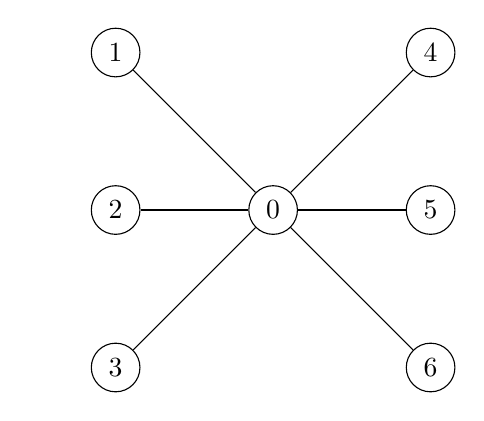
\begin{tikzpicture}
\node(pseudo) at (-1,0){};
\node(1) at (0,2)[shape=circle,draw]        {$1$};
\node(2) at (0,0)[shape=circle,draw]        {$2$};
\node(3) at (0,-2)[shape=circle,draw]        {$3$};
\node(0) at (2,0)[shape=circle,draw]        {$0$};
\node(4) at (4,2)[shape=circle,draw]        {$4$};
\node(5) at (4,0)[shape=circle,draw]        {$5$};
\node(6) at (4,-2)[shape=circle,draw]        {$6$};
\path [-]
  (1)      edge                 node [above]  {}     (0)
  (2)      edge                 node [above]  {}     (0)
  (3)      edge                 node [above]  {}     (0)
  (0)      edge                 node [above]  {}     (4)
  (0)      edge                 node [above]  {}     (5)
  (0)      edge                 node [above]  {}     (6);
\end{tikzpicture}

\begin{table}[H]
\begin{center}
\begin{tabular}{|l|l|}
\hline
Materias & Aulas en las que se puede dictar \\
\hline \hline
0 & (4, 3) \\ \hline
1 & (1, 5) \\ \hline
2 & (2, 3) \\ \hline
3 & (3) \\ \hline
4 & (1, 3) \\ \hline
5 & (2, 1) \\ \hline
6 & (3, 5) \\ \hline
\end{tabular}
\end{center}
\end{table}

Se ve que en el nodo número 0 no hay ninguna materia vecina que pueda ser dictada en el aula 4. Por lo tanto asignar a esta la misma aula será un coloreo valido para el nodo.
Obviamente existen casos en los que no se cumple esto y, sin embargo, la heurística nos puede devolver un resultado correcto. Para ejemplificar esto usaremos el grafo anterior
cambiando los colores posibles.

\begin{table}[H]
\begin{center}
\begin{tabular}{|l|l|}
\hline
Materias & Aulas en las que se puede dictar \\
\hline \hline
0 & (1, 3, 5) \\ \hline
1 & (1, 5) \\ \hline
2 & (1, 3) \\ \hline
3 & (3) \\ \hline
4 & (1, 3) \\ \hline
5 & (1, 5) \\ \hline
6 & (3, 5) \\ \hline
\end{tabular}
\end{center}
\end{table}

Podemos ver que no se cumple que halla alguna materia que tenga como aula posibles una que no pueda ser usada por las adyacentes. Sin embargo partiendo de cualquier nodo 
podemos colorear el grafo de la siguiente manera.

\begin{table}[H]
\begin{center}
\begin{tabular}{|l|l|}
\hline
Materias & Aula en que se dicta \\
\hline \hline
0 & (5) \\ \hline
1 & (1) \\ \hline
2 & (1) \\ \hline
3 & (3) \\ \hline
4 & (1) \\ \hline
5 & (1) \\ \hline
6 & (3) \\ \hline
\end{tabular}
\end{center}
\end{table}

Para mejorar un poco la heurística se decidió aplicar un pre-procesamiento de el grafo de coloreo que consiste en buscar todas las materias que solo puedan ser dictadas en una
aula y eliminar de sus adyacentes el aula como posible. Se repite esto hasta que no aparezcan más materias con esta característica. Se puede ver que este proceso no impide que 
para una instancia determinada donde se podría encontrar una solución esta no se alcance por la heurística constructiva golosa. Por otro lado hay algunos casos donde puede hacer
que en un caso particular se pueda encontrar un coloreo valido si se aplica en proceso anterior nombrado, y que antes no se encontraba.

\begin{tikzpicture}
\node(pseudo) at (-1,0){};
\node(0) at (0,2)[shape=circle,draw]        {$1$};
\node(1) at (0,0)[shape=circle,draw]        {$2$};
\node(2) at (0,-2)[shape=circle,draw]        {$3$};
\node(3) at (2,0)[shape=circle,draw]        {$0$};
\node(4) at (4,0)[shape=circle,draw]        {$4$};

\path [-]
  (0)      edge                 node [above]  {}     (3)
  (1)      edge                 node [above]  {}     (3)
  (2)      edge                 node [above]  {}     (3)
  (3)      edge                 node [above]  {}     (4);
\end{tikzpicture}


\begin{table}[H]
\begin{center}
\begin{tabular}{|l|l|}
\hline
Materias & Aulas en las que se puede dictar \\
\hline \hline
0 & (1, 2) \\ \hline
1 & (2, 3) \\ \hline
2 & (2, 4) \\ \hline
3 & (2, 5) \\ \hline
4 & (1) \\ \hline
\end{tabular}
\end{center}
\end{table}

Supongamos que comenzamos el BFS en el nodo 0. Entonces llegaremos al siguiente coloreo:

\begin{table}[H]
\begin{center}
\begin{tabular}{|l|l|}
\hline
Materias & Aula en las que se dictar \\
\hline \hline
0 & (1) \\ \hline
1 & (2) \\ \hline
2 & (2) \\ \hline
3 & (2) \\ \hline
4 & (1) \\ \hline
\end{tabular}
\end{center}
\end{table}

El cual no es valido. Sin embargo aplicando el pre-procesamiento anteriormente mencionado podemos alcanzar la siguiente solución.

\begin{table}[H]
\begin{center}
\begin{tabular}{|l|l|}
\hline
Materias & Aula en las que se dictar \\
\hline \hline
0 & (2) \\ \hline
1 & (3) \\ \hline
2 & (4) \\ \hline
3 & (5) \\ \hline
4 & (1) \\ \hline
\end{tabular}
\end{center}
\end{table}

La cual si es valida.

Obviamente también hay cirscuntancias donde la heurística va a fallar. Cambiando levemente el ejemplo anterior obtenemos lo siguiente.

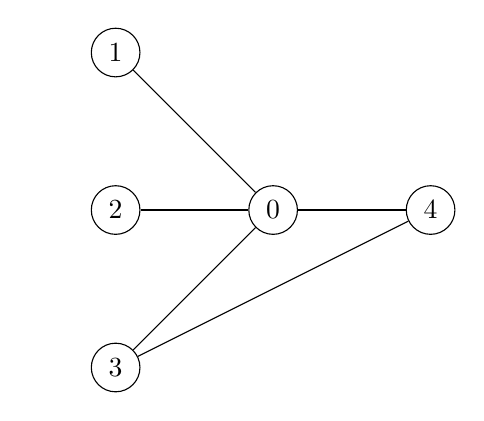
\begin{tikzpicture}
\node(pseudo) at (-1,0){};
\node(0) at (0,2)[shape=circle,draw]        {$1$};
\node(1) at (0,0)[shape=circle,draw]        {$2$};
\node(2) at (0,-2)[shape=circle,draw]        {$3$};
\node(3) at (2,0)[shape=circle,draw]        {$0$};
\node(4) at (4,0)[shape=circle,draw]        {$4$};

\path [-]
  (0)      edge                 node [above]  {}     (3)
  (1)      edge                 node [above]  {}     (3)
  (2)      edge                 node [above]  {}     (3)
  (3)      edge                 node [above]  {}     (4)
  (2)      edge                 node [above]  {}     (4);
\end{tikzpicture}


\begin{table}[H]
\begin{center}
\begin{tabular}{|l|l|}
\hline
Materias & Aulas en las que se puede dictar \\
\hline \hline
0 & (1, 2) \\ \hline
1 & (2, 5) \\ \hline
2 & (2, 3) \\ \hline
3 & (1, 5) \\ \hline
4 & (1, 5) \\ \hline
\end{tabular}
\end{center}
\end{table}

Hay que notar que el pre-procesamiento no realizara ningun cambio. El resultado de aplicar nuestra heurística es el siguiente:

\begin{table}[H]
\begin{center}
\begin{tabular}{|l|l|}
\hline
Materias & Aulas en las que se puede dictar \\
\hline \hline
0 & (1) \\ \hline
1 & (2) \\ \hline
2 & (2) \\ \hline
3 & (5) \\ \hline
4 & (5) \\ \hline
\end{tabular}
\end{center}
\end{table}

Y este es un coloreo invalido porque 3 y 4 son adyacentes y los dos estan coloreados con 5.

\subsection{Complejidad}

Tomamos n como la cantidad de vértices, m como la cantidad de aristas y c como la cantidad máxima de colores disponibles.

La complejidad del pre-procesamiento es el de recorrer cada uno de los vértices del grafo en busca de nodos con un solo color posible. Esto lo haremos, a lo sumo n veces.
En cada paso al encontrar una con un solo color posibles, procederemos a eliminar ese color de los adyacentes. El costo de eliminar un color de los adyacentes es en peor caso
O(c*n), mientras que recorrer el grafo a lo sumo n veces nos cuesta O($n^2$). En otras palabras la complejidad en peor caso del pre-procesamiento es de O($c*n^3$).

En cuanto a la complejidad del BFS, esta es la complejidad de recorrer el grafo con BFS multiplicado por lo que nos cuesta el coloreo en cada paso. BFS nos cuesta O($n*m$) en 
peor caso, mientras que buscar el color que menos aparece en los adyacentes nos cuesta O($n*c^2$) sumado a lo que nos cuesta eliminar el color elegido de los adyacentes lo que 
nos cuesta O($c*n$). En otras palabras la complejidad en peor caso del BFS es de O($n*m*(n*c^2 + c*n)$) = O($m*n^2*c^2$).

Por lo tango la complejidad en peor caso de nuestra heurística constructiva golosa es de O($m*n^3*c^2$).







\subsection{Experimentación}
